\documentclass[
  a4paper,
  % twocolumn,
  % draft
  ]{scrartcl}

% packages

  \usepackage{qbase}

  % extensions

    \bibliography{/Users/quirin/promo/bib/references}
    \usepackage{subcaption}

% new commands

  \renewcommand{\hw}[1]{\textbf{#1}}

  \newcommand{\lsil}[1]{\lstinline[language=Python]{#1}}
  \newcommand{\mtrc}[1]{\textcolor{blue}{#1}}

\begin{document}

% title

  \title{Social networks of lexical innovation}
  \subtitle{Investigating the diffusion of neologisms on Twitter}
  \author{Quirin Würschinger\\ LMU Munich}
  \maketitle

\listoftodos

\tableofcontents

% text body

  \cleardoublepage

\section{Introduction}

  The Corona virus has recently spread with shocking speed and has tragically affected the lives of people around the world. Its fatal consequences have demonstrated the devastating power of exponential contagion.  A leading research group of biologists analysing the spread of Corona have shown that the virus spreads supra-exponentially and they have likened its dynamics to the diffusion of cultural and linguistic innovations such as internet memes. \parencite{EandT2020} Does this confirm the popular perception that certain cultural and linguistic innovations \enquote{go viral}, after all?

  Societies constantly evolve, new products and practices emerge and speakers continually invent and adopt new words which diffuse through social networks of communicative interaction. Influential models in sociolinguistics like the S-curve model \parencite{Milroy1992} and its compatibility with economic models \parencite{Rogers1962} suggest commonalities between the diffusion of cultural and linguistic innovations. These models assume that the diffusion of linguistic innovations across social networks follows universal trajectories and that rates of diffusion depend on sociolinguistic dynamics such as network density and the presence or absence of weak ties \parencite{Granovetter1977}.

  Unlike research on biological and cultural diffusion processes, sociolinguistic research has only fairly recently been provided with datasets that are suitable for large-scale, data-based approaches and that contain the necessary information to study these phenomena empirically using social network analyses.

  The technological innovation of social media platforms like Twitter and the increasing availability of linguistic data from these sources for academic research allow for large-scale usage-based investigations of authentic language use.

  The informal nature and the sheer size of these data have promoted significant advances in the study of new words, as neologisms are often propagated via social media channels and as their inherently low frequency of occurrence requires large corpora. In contrast to modern web corpora, which share these features, the availability of metadata about speakers and their interactions has been particularly important for the advancement of sociolinguistic research.

  For example, recent sociolinguistic work on lexical innovation has used social media data to gain insights about general trajectories \parencite{Nini2017} and geographical patterns \parencite{Eisenstein2014,Grieve2017,Grieve2018} of diffusion and about factors that influence whether new words spread successfully \parencite{Grieveforthcoming}.

  new methods: social networks

    The study of social networks has had a long research tradition in sociolinguistics and has shaped current models of diffusion (e.g. \cite{Milroy1985}). However, large-scale empirical corpus studies using social network analysis have only recently become feasible in the field of sociolinguistics.

      promising in other fields: agent-based modeling
      also promising for lexical innovation
      not been done enough
      I will do it

  \todo{
    impact of social media
      social fabric: elections, press, influencers
      how we communicate: fake news
      language system: blends, acronyms, hashtags
  }

  This paper presents an empirical approach to investigate these phenomena by studying the trajectory and sociolinguistic dynamics of how new words diffuse across social networks on Twitter.

  Section X will present the theoretical framework for modelling the diffusion of new words ... and operationalization
  Section X will indicate the data and methods I use for my empirical investigation
  Section

\section{Theoretical background}

    \hw{Research question}: How do new words diffuse and become conventional lexical items in a language system?

  \subsection{Research perspectives}

    A substantial body of linguistic research has tackled this question from different \hw{perspectives}. \parencite[16]{Schmid2016}

    From a \hw{structural} perspective, main areas of interest include which word-formation processes are involved in forming new words, whether they are formally and semantically transparent, whether they show variation and change in the process of lexicalization and which status the resulting neologisms have in the language system (institutionalization). (e.g. \cite{Bauer1983,Lipka2005}

    \hw{Cognitive} perspectives focus on how individuals process and store lexical innovations. Speakers generally use new words when they experience a communicative need to talk about entities or practices that cannot be expressed by their language's inventory of conventional words yet. In order for neologisms to successfully diffuse, speakers need to successfully negotiate their meaning (co-semiosis) in discourse, others need to adopt the behaviour of using these words (co-adaption). Continued exposure and use of new words can then lead to the entrenchment of new words in the mental lexicon of speakers. \parencite{Schmid2008}

    \hw{Sociolinguistic} perspectives transcend the level of the individual to study the diffusion of new words across speakers. The diffusion of lexical innovations is commonly seen as successful when the majority of the speech community has accepted a new word as a conventional lexical unit that can and is being used in communicative practice.

  \subsection{The S-curve model}

    \hw{S-curve models} of linguistic change \parencite{Labov2007,Milroy1992,Nevalainen2015} assume universal sociolinguistic dynamics for the diffusion of linguistic innovations.

    \begin{easylist}[itemize]

      # The \hw{trajectory} of spread is expected to follow an S-curve shape, with low rates of diffusion in early stages, followed by a period of accelerating spread with a tipping point at the mid point in the diffusion curve after which diffusion slows down and the curve flattens towards the end of the diffusion process.

      # These temporal trajectories are assumed to correspond to the \hw{sociolinguistic dynamics} of which individuals and groups interact with each other and adopt the target innovation.

        ## In the \hw{first stage} of slow diffusion only a small number of early adopters take up the innovative words. The individuals who use the new word typically form dense networks connected by strong ties. The structure of tight-knit communities of potentially like-minded individuals of similar backgrounds facilitates the successful negotiation of meaning (co-semiosis) of new words. High rates of interactions in these communities leads to high rates of exposure for individuals, which fosters co-adaption, entrenchment and usualization of new words in these communities.

        ## In cases of successful diffusion the initial stages are followed by an \hw{acceleration in spread} when new words increasingly reach speakers outside these tight-knit communities via weak ties \parencite{Granovetter1977}. Rates of diffusion increase substantially when speakers that are not part of the initial group of early adopters start to accomodate the new words, allowing the innovations to reach a broader spectrum of the speech community.

        ## In \hw{later stages}, rates of diffusion slow down again as the majority of the speech community has already adopted the new words while smaller pockets speakers remain reluctant to take up the new words.

      # S-curve models have mainly been applied to the \hw{linguistic domains} of phonology and syntax. Fundamental differences between lexemes and linguistic items on other levels such as phonemes and grammatical constructions might affect whether the validity and reliability of such models for \emph{lexical} innovation.

        ## For example, grammatical constructions such as the \ol{going to} future used to express a speaker's future intention serve to fulfill relatively abstract communicative needs that remain stable over time. By contrast, on the lexical level, linguistic innovations are typically tied to concrete cultural referents such as products and practices whose conceptual relevance is much more volatile over time. For example, many lexical innovations such as \ol{millennium bug} denoting the fear of a computer crash at the beginning of the new millennium can show high rates of diffusion and become entrenched and conventional among the majority of the speech community. Without continual conceptual relevance in public discourse, however, these words fail pass on to the next generation of speakers. S-curves are commonly assumed to be found when linguistic innovations compete for \hw{\enquote{semantic carrying capacity}} \parencite{Nini2017}, however, in many if not most cases of \emph{lexical} innovation the conceptual carrying capacity is far from stable over time which represents a critical deviation from the traditional assumptions behind S-curves in language change.

        ## However, the generally strong theoretical and empirical basis of the S-curve model for language innovation and change, also from studies on the diffusion of cultural innovations \parencite{Rogers1962}, and the precise formulation of the sociolinguistic dynamics underlying different phases of diffusion still make it an attractive \hw{blueprint} for the empirical study of the sociolinguistic diffusion of lexical innovations.

    \end{easylist}

  \subsection{Empirical approaches}

    \begin{easylist}[itemize]
      # Previous work has produced some important insights.
      # I focus on the sociolinguistic dimension of lexical innovation in this paper.
      # Previous empirical approaches have been limited in studying this because of the lack of information regarding the sociolinguistic dynamics of the spread of new words: how many speakers are affected? how are they interacting?
    \end{easylist}

    Overview of previous approaches

      \begin{easylist}[itemize]
        # traditional corpora \parencite{Elsen2004}
        # web corpora \parencite{Renouf2006,Kerremans2012,Lemnitzer,Gerard2017,Cartier2017}
          ## linguistic creativity and innovation happen there
          ## big amounts of data
            ### big neologism samples
            ### big corpora (low-frequency nature of neologisms)
          ## more informal sources
        # social media corpora \cite{Grieve2016,Eisenstein2014}
          # hotbed
          # driving force
          # social network information
            ## users
            ## community characteristics
            ## influencers
      \end{easylist}

  \subsection{Current framework: the EC-Model (Schmid 2020)}
    \nocite{Schmid2020}

    The EC-Model integrates both structural, cognitive and sociolinguistic perspectives on language structure, variation and change.

    \hw{Entrenchment}: individuals

    \hw{Conventionalization}: society, sociolinguistics $\rightarrow$ focus of this paper

    \hw{Usualization}

    \hw{Diffusion}

      definition

  \subsection{Operationalization}

    \begin{easylist}[itemize]
      # going beyond frequency
      # sociolinguistic dynamics
        ## number of users
        ## social network characteristics
        ## influencers
    \end{easylist}

\section{Data and methods}

  \subsection{Data}

    \begin{easylist}[itemize]
      # corpus
        ## longitudinal: retrospective, starting from early attestations
        ## big data
        ## social network information
      # sample
        ## basis: bottom-up selection by NeoCrawler \parencite{Kerremans2018}
        ## covering candidates from clusters found in earlier empirical work \parencite{Kerremans2015}
          ### no diffusion
          ### topical
          ### recurrent
          ### advanced
        ## extension
          ### reasonably successful: e.g. technical innovations like \ol{blockchain}
          ### sociolinguistically interesting: e.g. political terms such as \ol{covfefe}
    \end{easylist}

  \subsection{Method: social network analysis}

    \begin{easylist}[itemize]
      # basis for networks: interactions between users
        ## mentions
        ## retweets
      # anatomy of a tweet
      # network structure
        ## nodes: users
        ## edges: interactions
    \end{easylist}

\section{Sample}

  \subsection{Neologism candidates}

    \begin{easylist}[itemize]

      # previous categorization \parencite{Kerremans2015}
        ## no diffusion
        ## topical
        ## recurrent
        ## advanced

      # dimensions

        ## overall degree of diffusion (synchronic): successful vs. unsuccessful: \mtrc{usage frequency}, \mtrc{degree centralization}
          ### no success
          ### limited
          ### advanced

        ## temporal dynamics of diffusion (diachronic)
          ## stability: stable vs. topical \mtrc{coefficient of variation}
          ## trend
            ## diffusion: increasing degree of diffusion
            ## centralization: decreasing degree of diffusion
          ## speed

    \end{easylist}

  \subsection{Case studies}

    \begin{easylist}[itemize]

      # criteria

        ## covering clusters of neolgism candidates
        ## frequency counts comparable

      # cases \parencite{Kerremans2015}
        ## no diffusion: \ol{microflat}
        ## limited
          ### topical: \ol{poppygate}
          ### centralized: \ol{alt-left}
          ### decreasing: \ol{solopreneur}
        ## advanced diffusion:
          ### advanced: \ol{upcycling}
          ### increasing: \ol{hyperlocal}

    \end{easylist}

\section{Frequency}

  \begin{easylist}[itemize]

    # Frequency is usually taken as the measure to approximate the degree of conventionality and entrenchment of linguistic entities.

    # There are a number of underlying assumptions.

      ## speech community: frequency = conventionality
        ### high freq. = majority of speakers show entrenchment
      ## individuals: exposure $\rightarrow$ entrenchment

    # problems

      ## temporal dynamics (e.g. \ol{millenium bug})
      ## output != input ~\parencite{Stefanowitsch2017}
      ## high freq != many speakers
      ## many speakers != \enquote{majority of the speech community}

  \end{easylist}

  \subsection{Overall degree of diffusion}

    \begin{figure}[H]
      \caption{Cumulative counts for unique speakers that have used the target neologisms.}
      \centering
      \begin{subfigure}{.45\linewidth}
        \caption{\ol{ghosting}}
        \centering
        \includegraphics[width=\linewidth, height=.8\textheight, keepaspectratio]{/Users/quirin/promo/sna/out/users/uu_ghosting.pdf}
      \end{subfigure}
      \begin{subfigure}{.45\linewidth}
        \caption{\ol{lituation}}
        \centering
        \includegraphics[width=\linewidth, height=.8\textheight, keepaspectratio]{/Users/quirin/promo/sna/out/users/uu_lituation.pdf}
      \end{subfigure}

      \begin{subfigure}{.45\linewidth}
        \caption{\ol{alt-left}}
        \centering
        \includegraphics[width=\linewidth, height=.8\textheight, keepaspectratio]{/Users/quirin/promo/sna/out/users/uu_alt-left.pdf}
      \end{subfigure}
      \begin{subfigure}{.45\linewidth}
        \caption{\ol{solopreneur}}
        \centering
        \includegraphics[width=\linewidth, height=.8\textheight, keepaspectratio]{/Users/quirin/promo/sna/out/users/uu_solopreneur.pdf}
      \end{subfigure}
    \end{figure}

  \subsection{Temporal dynamics}

    \subsubsection{Coefficient of variation}

      \begin{easylist}[itemize]
        # most volatile candidates: \ol{poppygate}, \ol{burkini} etc.
        # will be excluded from in-depth analyses
      \end{easylist}

  \subsection{Speaker counts}

      I will go beyond frequency and look into the sociolinguistic dynamics more closely

      \begin{easylist}[itemize]
        # sociolinguistic dynamics of diffusion over time
        # sociolinguistic conventionality status of neologism
      \end{easylist}

\section{Diffusion over time}

  \subsection{Advanced: \ol{ghosting}}

    \begin{figure}[H]
      \caption{Usage frequency for \ol{ghosting}.}
      \centering
      \includegraphics[width=\linewidth, height=.8\textheight, keepaspectratio]{/Users/quirin/promo/sna/out/uses/ui_ghosting_time.pdf}
    \end{figure}

    \begin{figure}[H]
      \caption{Social network of diffusion for \ol{ghosting} over time.}
      \centering
      \begin{subfigure}{.45\linewidth}
        \caption{First stage}
        \centering
        \includegraphics[width=\linewidth, height=\textheight, keepaspectratio]{/Users/quirin/promo/sna/gephi/plots/ghosting_one.pdf}
      \end{subfigure}
      \begin{subfigure}{.45\linewidth}
        \caption{Second stage}
        \centering
        \includegraphics[width=\linewidth, height=\textheight, keepaspectratio]{/Users/quirin/promo/sna/gephi/plots/ghosting_two.pdf}
      \end{subfigure}\\
      \begin{subfigure}{.45\linewidth}
        \caption{Third stage}
        \centering
        \includegraphics[width=\linewidth, height=\textheight, keepaspectratio]{/Users/quirin/promo/sna/gephi/plots/ghosting_three.pdf}
      \end{subfigure}
      \begin{subfigure}{.45\linewidth}
        \caption{Fourth stage}
        \centering
        \includegraphics[width=\linewidth, height=\textheight, keepaspectratio]{/Users/quirin/promo/sna/gephi/plots/ghosting_four.pdf}
      \end{subfigure}
    \end{figure}

  \subsection{Advanced: \ol{upcycling}}

    \begin{figure}[H]
      \caption{Usage frequency for \ol{upcycling}.}
      \centering
      \includegraphics[width=\linewidth, height=.8\textheight, keepaspectratio]{/Users/quirin/promo/sna/out/uses/ui_upcycling_time.pdf}
    \end{figure}

    \begin{figure}[H]
      \caption{Social network of diffusion for \ol{upcycling} over time.}
      \centering
      \begin{subfigure}{.45\linewidth}
        \caption{First stage}
        \centering
        \includegraphics[width=\linewidth, height=\textheight, keepaspectratio]{/Users/quirin/promo/sna/gephi/plots/upcycling_one.pdf}
      \end{subfigure}
      \begin{subfigure}{.45\linewidth}
        \caption{Second stage}
        \centering
        \includegraphics[width=\linewidth, height=\textheight, keepaspectratio]{/Users/quirin/promo/sna/gephi/plots/upcycling_two.pdf}
      \end{subfigure}\\
      \begin{subfigure}{.45\linewidth}
        \caption{Third stage}
        \centering
        \includegraphics[width=\linewidth, height=\textheight, keepaspectratio]{/Users/quirin/promo/sna/gephi/plots/upcycling_three.pdf}
      \end{subfigure}
      \begin{subfigure}{.45\linewidth}
        \caption{Fourth stage}
        \centering
        \includegraphics[width=\linewidth, height=\textheight, keepaspectratio]{/Users/quirin/promo/sna/gephi/plots/upcycling_four.pdf}
      \end{subfigure}
    \end{figure}

  \subsection{Increasing diffusion: \ol{lituation}}

    \begin{figure}[H]
      \caption{Usage frequency of \ol{lituation} over time.}
      \centering
      \includegraphics[width=\linewidth, height=.8\textheight, keepaspectratio]{/Users/quirin/promo/sna/out/uses/ui_lituation_time.pdf}
    \end{figure}

    \begin{figure}[H]
      \caption{Social network of diffusion for \ol{lituation} over time.}
      \centering
      \begin{subfigure}{.45\linewidth}
        \caption{First stage}
        \centering
        \includegraphics[width=\linewidth, height=\textheight, keepaspectratio]{/Users/quirin/promo/sna/gephi/plots/lituation_one.pdf}
      \end{subfigure}
      \begin{subfigure}{.45\linewidth}
        \caption{Second stage}
        \centering
        \includegraphics[width=\linewidth, height=\textheight, keepaspectratio]{/Users/quirin/promo/sna/gephi/plots/lituation_two.pdf}
      \end{subfigure}\\
      \begin{subfigure}{.45\linewidth}
        \caption{Third stage}
        \centering
        \includegraphics[width=\linewidth, height=\textheight, keepaspectratio]{/Users/quirin/promo/sna/gephi/plots/lituation_three.pdf}
      \end{subfigure}
      \begin{subfigure}{.45\linewidth}
        \caption{Fourth stage}
        \centering
        \includegraphics[width=\linewidth, height=\textheight, keepaspectratio]{/Users/quirin/promo/sna/gephi/plots/lituation_four.pdf}
      \end{subfigure}
    \end{figure}

  \subsection{Centralized use: \ol{alt-left}}

    \begin{figure}[H]
      \caption{Usage frequency of \ol{alt-left} over time.}
      \centering
      \includegraphics[width=\linewidth, height=.8\textheight, keepaspectratio]{/Users/quirin/promo/sna/out/uses/ui_alt-left_time.pdf}
    \end{figure}

    \begin{figure}[H]
      \caption{Social network of diffusion for \ol{alt-left} over time.}
      \centering
      \begin{subfigure}{.45\linewidth}
        \caption{First stage}
        \centering
        \includegraphics[width=\linewidth, height=\textheight, keepaspectratio]{/Users/quirin/promo/sna/gephi/plots/alt-left_one.pdf}
      \end{subfigure}
      \begin{subfigure}{.45\linewidth}
        \caption{Second stage}
        \centering
        \includegraphics[width=\linewidth, height=\textheight, keepaspectratio]{/Users/quirin/promo/sna/gephi/plots/alt-left_two.pdf}
      \end{subfigure}\\
      \begin{subfigure}{.45\linewidth}
        \caption{Third stage}
        \centering
        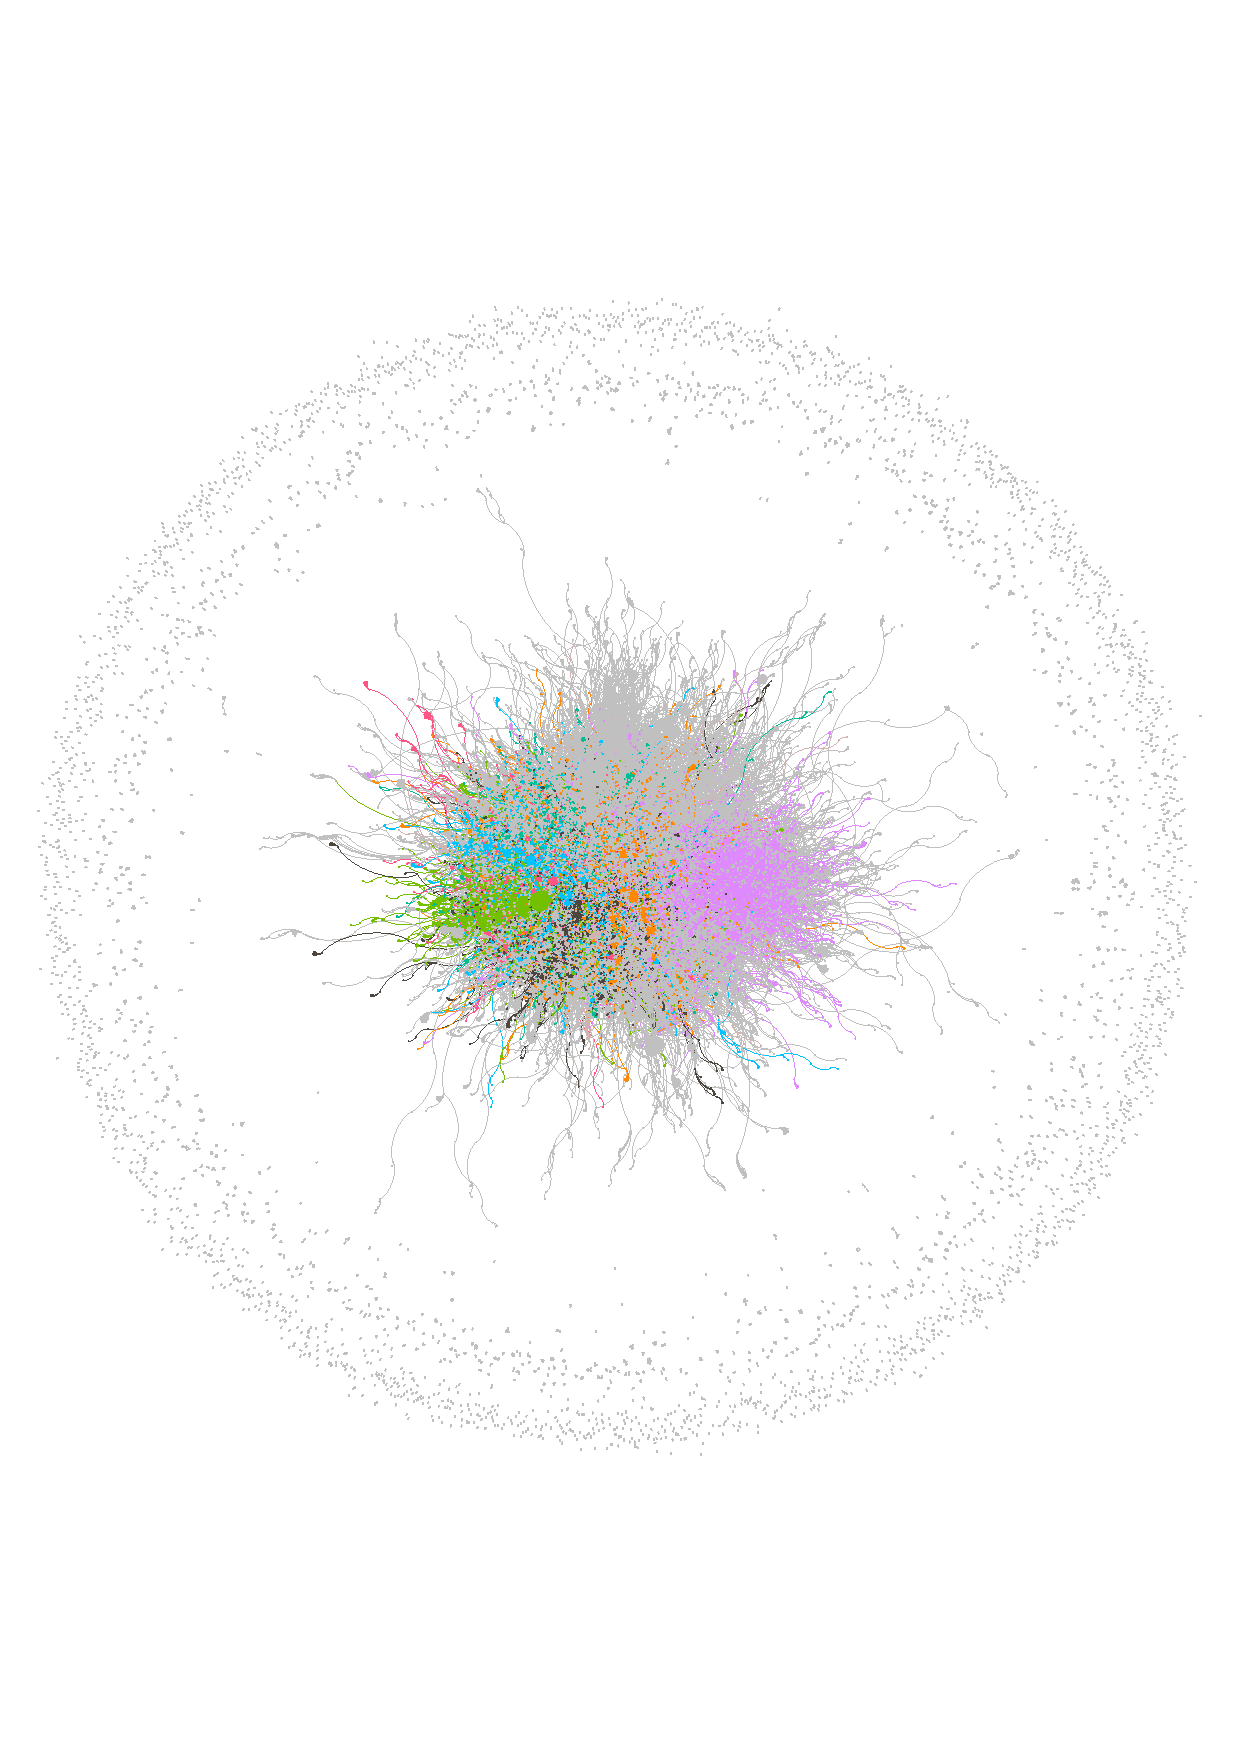
\includegraphics[width=\linewidth, height=\textheight, keepaspectratio]{/Users/quirin/promo/sna/gephi/plots/alt-left_three.pdf}
      \end{subfigure}
      \begin{subfigure}{.45\linewidth}
        \caption{Fourth stage}
        \centering
        \includegraphics[width=\linewidth, height=\textheight, keepaspectratio]{/Users/quirin/promo/sna/gephi/plots/alt-left_four.pdf}
      \end{subfigure}
    \end{figure}

  \subsection{Narrowing: \ol{solopreneur}}

    \begin{figure}[H]
      \caption{Usage frequency of \ol{solopreneur} over time.}
      \centering
      \includegraphics[width=\linewidth, height=.8\textheight, keepaspectratio]{/Users/quirin/promo/sna/out/uses/ui_solopreneur_time.pdf}
    \end{figure}

    \begin{figure}[H]
      \caption{Social network of diffusion for \ol{solopreneur} over time.}
      \centering
      % \begin{subfigure}{.45\linewidth}
      %   \caption{First stage}
      %   \centering
      %   \includegraphics[width=\linewidth, height=\textheight, keepaspectratio]{/Users/quirin/promo/sna/gephi/plots/solopreneur_one.pdf}
      % \end{subfigure}
      % \begin{subfigure}{.45\linewidth}
      %   \caption{Second stage}
      %   \centering
      %   \includegraphics[width=\linewidth, height=\textheight, keepaspectratio]{/Users/quirin/promo/sna/gephi/plots/solopreneur_two.pdf}
      % \end{subfigure}\\
      % \begin{subfigure}{.45\linewidth}
      %   \caption{Third stage}
      %   \centering
      %   \includegraphics[width=\linewidth, height=\textheight, keepaspectratio]{/Users/quirin/promo/sna/gephi/plots/solopreneur_three.pdf}
      % \end{subfigure}
      % \begin{subfigure}{.45\linewidth}
      %   \caption{Fourth stage}
      %   \centering
      %   \includegraphics[width=\linewidth, height=\textheight, keepaspectratio]{/Users/quirin/promo/sna/gephi/plots/solopreneur_four.pdf}
      % \end{subfigure}
    \end{figure}

  \subsection{Overall diachronic development for case studies}

    \begin{figure}[H]
      \caption{Degree centralization over time for case study words.}
      \centering
      \includegraphics[width=\linewidth, height=.8\textheight, keepaspectratio]{/Users/quirin/promo/sna/out/cases_cent_diac.pdf}
    \end{figure}

\section{Full sample}

  \subsection{Diachronic development}

    \begin{figure}
      \caption{Degree centralization over time for the full sample.}
      \centering
      \includegraphics[width=\linewidth, height=.8\textheight, keepaspectratio]{/Users/quirin/promo/sna/out/full_cent_diac.pdf}
    \end{figure}

  \subsection{Biggest changes}

    \begin{easylist}[itemize]
      # increasing diffusion
      # centralization
    \end{easylist}

\section{Networks vs. frequency}

  \subsection{Plots}

    \begin{figure}
      \centering
      \begin{subfigure}{.45\linewidth}
        \caption{Full sample.}
        \centering
        \includegraphics[width=\linewidth, height=.8\textheight, keepaspectratio]{/Users/quirin/promo/sna/out/full_cent_freq_overall.pdf}
      \end{subfigure}
      \begin{subfigure}{.45\linewidth}
        \caption{Case studies.}
        \centering
        \includegraphics[width=\linewidth, height=.8\textheight, keepaspectratio]{/Users/quirin/promo/sna/out/cases_cent_freq_overall.pdf}
      \end{subfigure}
    \end{figure}

  \subsection{Correlation}

  \subsection{Grouping and interpretation}

    Divergences between frequency and network analysis

      \begin{easylist}[itemize]
        # advanced
        # topical
        # little dispersion
          ## political camps:
            ### propaganda: \ol{alt-right}, \ol{alt-left}, \ol{covfefe}, \ol{birther}
            ### Brexit terms: \ol{Brexiteer}, \ol{Brexiter}, \ol{Brexit}
          ## technical
      \end{easylist}

    $\rightarrow$ case studies

\section{Conclusion}

  \begin{easylist}[itemize]
    # going beyond frequency is important
  \end{easylist}

% bibliography

  \printbibliography

\end{document}
